% Тут используется класс, установленный на сервере Papeeria. На случай, если
% текст понадобится редактировать где-то в другом месте, рядом лежит файл matmex-diploma-custom.cls
% который в момент своего создания был идентичен классу, установленному на сервере.
% Для того, чтобы им воспользоваться, замените matmex-diploma на matmex-diploma-custom
% Если вы работаете исключительно в Papeeria то мы настоятельно рекомендуем пользоваться
% классом matmex-diploma, поскольку он будет автоматически обновляться по мере внесения корректив
%

% По умолчанию используется шрифт 14 размера. Если нужен 12-й шрифт, уберите опцию [14pt]
%\documentclass[14pt]{matmex-diploma}
\documentclass[14pt]{matmex-diploma-custom}

\begin{document}
% Год, город, название университета и факультета предопределены,
% но можно и поменять.
% Если англоязычная титульная страница не нужна, то ее можно просто удалить.
\filltitle{ru}{
    chair              = {Математическое обеспечение и администрирование информационных систем\\Системное программирование},
    title              = {Разработка алгоритмов скаффолдинга при помощи дополнительной геномной информации},
    % Здесь указывается тип работы. Возможные значения:
    %   coursework - Курсовая работа
    %   diploma - Диплом специалиста
    %   master - Диплом магистра
    %   bachelor - Диплом бакалавра
    type               = {bachelor},
    position           = {студента},
    group              = 444,
    author             = {Клещин Антон Сергеевич},
    supervisorPosition = {доц. каф. СП, к.т.н.},
    supervisor         = {Литвинов Ю.\,В.},
    supervisorPositionx   = {доц. каф. СМ, к.ф.-м.н.},
    supervisorx           = {Коробейников А.\,И.},
    supervisorPositiony   = {Научный сотрудник Центра алгоритмической биотехнологии СПбГУ},
    supervisory           = {Пржибельский А.\,Д.},
    reviewerPosition  = {Аспирант},
    reviewer          = {Мелешко Д.\,А.},
%   university         = {Санкт-Петербургский Государственный Университет},
%   faculty            = {Математико-механический факультет},
%   city               = {Санкт-Петербург},
%   year               = {2013}
}
\filltitle{en}{
    chair              = {Software and Administration of Information Systems \\ Software Engineering},
    title              = {Development of scaffolding algorithms using additional genomic information},
    type               = {bachelor},
    author             = {Anton Kleshchin},
    supervisorPosition = {C.Sc., Associate Professor},
    supervisor         = {Yurii Litvinov},
    supervisorPositionx   = {Ph.D., Associate Professor},
    supervisorx           = {Anton Korobeynikov},
    supervisorPositiony   = {Research Fellow at the Center for Algorithmic Biotechnology SPbU},
    supervisory           = {Andrey Prjibelski},
    reviewerPosition  = {PhD Candidate},
    reviewer          = {Dmitrii Meleshko},
}
\maketitle
\tableofcontents
\setcounter{secnumdepth}{4}
%==============================================================================
% У введения нет номера главы
\section*{Введение}
Сборка геномов является одной из важнейших задач биоинформатики. За многие годы учёным уже удалось собрать, а затем и расшифровать большое количество геномов. Несмотря на это, автоматическая реконструкция генома всё ещё остаётся сложной вычислительной задачей \cite{sohn2018present, art:collins2018challenge}. 

Обычно сборка генома происходит из ридов (англ. reads) --- фрагментов ДНК, которые получаются в результате секвенирования, а результатом являются контиги (англ. contigs, восстановленные части ДНК из ридов) или скаффолды (англ. scaffolds, восстановленные части ДНК с пропусками известной длины). Но если в дополнение к ридам кто-то даст последовательность, которая очень похожа на часть генома, например, ранее собранный контиг или скаффолд, то, разумеется, этой новой информацией захочется воспользоваться.

За время существования биоинформатики улучшались старые и появлялись новые методы и алгоритмы сборки геномных последовательностей \cite{art:simpson2015theory}. Накопилось огромное количество данных, полученных в результате ручной реконструкции. Всю эту информацию можно переиспользовать для получения более качественных новых результатов.

Помимо этого появилось огромное множество геномных ассемблеров \cite{art:zimin2013masurca, art:sommer2007minimus, art:georganas2015hipmer, art:batzoglou2002arachne, art:abu2015spaler}, которые используют всевозможные подходы и идеи решения проблем, появляющихся во время реконструкции генома. Эти идеи и подходы срабатывают с разным уровнем успеха. Если объединить результаты сборки разных ассемблеров в виде дополнительных данных для новой сборки, то можно можно получить результаты, недоступные ни одному отдельно взятому ассемблеру.

Можно использовать уже существующие результаты сборок одних геномов для сборки похожих геномов. В клетках постоянно происходят мутации, появляются новые штаммы бактерий и вирусов, а различные штаммы довольно похожи друг на друга большими участками генома даже при наличии структурных изменений. Например, E.coli K-12 можно собрать с помощью сборки E.coli DH-10, ведь у них есть сегмент генома, сопоставимый с десятой частью длины всего генома и похожий на 99\%.

Кроме того, можно не ограничиваться сборками бактерий по одной. Метагеномика --- направление геномики, в котором рассматриваются ДНК не отдельного организма, а сразу множества. При таком подходе часто уже имеется некоторая информация о бактериях, чьи нуклеотидные последовательности ДНК присутствуют в исследуемых данных. Эти бактерии также уже могут быть хорошо исследованы раньше, поэтому использование их референсных геномов может существенно упростить исследование остальных бактерий. 

\begin{sloppypar}
В мире существует огромное множество геномных ассемблеров, которые специализируются на сборке некоторых классов организмов из определённых типов ридов. Например, есть геномный ассемблер SPAdes \cite{art:SPAdes}, разрабатываемый Центре алгоритмической биотехнологии при \mbox{СПбГУ}. Он поддерживает одновременное использование большинства типов ридов для реконструкции генома. Помимо этого он является одним из лучших ассемблеров, специализирующихся на сборке геномов бактерий \cite{art:assemblers_cmp}. Несмотря на то, что SPAdes уже позволял использовать контиги в качестве входных данных, они использовались далеко не самым эффективным образом, потому что использовался алгоритм, разработанный для длинных ридов, а не для для контигов.
\end{sloppypar}

Итак, оказывается актуальной разработка нового алгоритма скаффолдинга, поддерживающего контиги.

%==============================================================================
\section{Постановка задачи}
Целью данной дипломной работы является добавление поддержки контигов в качестве входных данных для геномного ассемблера SPAdes. Для достижения этой цели были сформулированы следующие задачи.
\begin{itemize}
    \item Разработка алгоритма скаффолдинга, использующего
контиги.
    \item Реализация расширения для геномного ассемблера SPAdes.
    \item Тестирование алгоритма на известных геномах.
\end{itemize}

%==============================================================================
\section{Обзор предметной области}
\subsection{Представление генома}
Большинство природных ДНК состоит из двух скрученных спиралей, к которым крепятся молекулы, называемые нуклеотидами \cite{art:Watson}. Всего в спиралях присутствует четыре вида нуклеотида: аденин (A), цитозин (C), гуанин (G), тимин (T). Двойная спираль ДНК может иметь либо линейную структуру, либо кольцевую. Одноцепочечную ДНК содержат лишь некоторые вирусы и бактериофаги. При этом известно, что одна спираль полностью задаёт другую: напротив каждого нуклеотида из одной цепочки стоит комплементарный ей из другой. Для аденина это тимин, а для гуанина --- цитозин.

Таким образом можно считать, что ДНК состоит из двух комплементарных строк над алфавитом из четырёх букв. Длину подстрок принято измерять в спаренных основаниях (англ. base pair, \textbf{bp}), которые эквивалентны одному символу строки.

\subsection{Сборка геномов}
Современные технологии не могут считывать всю ДНК за раз, поэтому в результате секвенирования получается множество фрагментов ДНК, называемых ридами. В зависимости от используемой технологии, длина ридов может быть разной, но самые популярные технологии умеют получать цепочки нуклеотидов порядка 100-200 bp, в то время как, например, длина генома у бактерий измеряется в миллионах bp. К сожалению, при секвенировании происходят ошибки, поэтому ДНК читается несколько раз, чтобы в перекрытии каждого нуклеотида результирующим набором ридов было больше правильных значений, чем ошибочных.

Задачей ассемблера является восстановление одной из нитей спирали ДНК по ридам. Обычно удаётся  восстановить лишь фрагменты ДНК, которые являются либо контигами, либо скаффолдами. Их отличие в том, что в случае скаффолдов допускаются подстроки, в которых нуклеотиды неизвестны, что даёт дополнительную информацию в виде расстояния между контигами и их порядка следования в геноме.

\subsection{Граф де Брюйна}
Методы сборки ридов в контиги далеко шагнули вперёд. В некоторых современных ассемблерах и, в частности, в SPAdes используется подход, основанный на графе де Брюйна (англ. de Bruijn graph) \cite{art:Pevzner}. Этот граф строится по следующим принципам: берётся набор входных строк и выделяется из них множество всевозможных подстрок длины k+1 (k+1-меры). Тогда направленными рёбрами будут выступать k+1-меры. Вершинами же будут k-меры, полученные уже из k+1-меров и выступающие в роли перекрытия между ними. Соответственно, к вершине подсоединяются рёбра тем концом, который содержит k-мер вершины. Пример графа можно видеть на рисунке \ref{fig:debruijn}.

\begin{figure}[h]
	\centering
	\includegraphics[scale=0.3]{debruijn.png}
	\caption{Граф де Брюйна для строки ACGTCCGTAA с параметром ${k=2}$.}
	\label{fig:debruijn}
\end{figure}

Изначально предполагалось, что для того, чтобы собрать исходный геном, требуется найти в графе де Брюна Эйлеров цикл или путь с учётом кратности рёбер, которая считается на основе покрытия рёбер ридами \cite{art:disser_andrey}. Так как количество действий, требуемых для нахождения Эйлерова цикла, пропорционально количеству вершин в графе, то этот метод позволяет собирать геномы, состоящих из миллиардов ридов. Но, к сожалению, этот метод в чистом виде работает только в рамках трёх допущений:
\begin{enumerate}
    \item все k-меры из генома присутствуют в ридах;
    \item все k-меры не содержат ошибок;
    \item геном состоит из одной круговой хромосомы;
\end{enumerate}

В реальности же это очень сильные ограничения, с которыми, правда, можно бороться \cite{art:Compeau}.

\subsection{Архитектура SPAdes}
Конвейер сборки в SPAdes состоит из набора этапов, которые выполняются один или несколько раз в некотором порядке, зависящем от типа сборки. Здесь мы рассмотрим только несколько из этапов, важных для дальнейшего повествования.

%\paragraph{Построение графа де Брюйна}\mbox{}
\subsubsection{Построение графа де Брюйна}

Первым этапом является построение графа де Брюйна. Существует много типов ридов, и для каждого из них применяются свои подходы при сборке генома \cite{art:ex:Ghurye2, art:ex:Chaisson, art:ex:Sedlazeck, art:ex:Ghurye1}.
%\cite{art:ex:Nagarajan, art:ex:Ghurye2, art:ex:Miller, art:ex:Simpson, art:ex:Schatz, art:ex:Alkan, art:ex:Chaisson, art:ex:Sedlazeck, art:ex:Ghurye1}.
В SPAdes для создания графа де Брюйна используются те типы ридов, вероятность ошибки в которых невысока и количество неверных нуклеотидов составляет обычно не более одного процента от длины рида.

При построении графа также считается покрытие рёбер ридами. Так как ридов, используемых при построении графа, очень много, а количество ошибок в них минимально, то у правильных рёбер (то есть тех рёбер, которые должны войти в ответ) покрытие будет высокое. В то же время любая ошибка в риде породит ответвление, в котором рёбра будут иметь очень низкое покрытие. Этот факт используется на следующем этапе сборки генома, который называется упрощением.

%\paragraph{Упрощение графа}\mbox{}
\subsubsection{Упрощение графа}

Упрощение графа де Брюйна до графа сборки необходимо по нескольким причинам, которые описаны в работе \cite{art:disser_andrey}. Одной из главных частей упрощения, на которой основывается алгоритм из данной работы, является удаление рёбер с низким покрытием, то есть тех, которые, скорее всего, являются ошибочными. Но это удаление ведёт себя довольно хитрым образом, а именно: оно не всегда полностью теряет информацию о существовании удаляемого ребра. Перед непосредственным удалением алгоритм пытается найти другое ребро в графе, которое исходит из вершин, соединённых с удаляемым ребром, и которое максимально на него похоже. Если подходящее ребро находится, то в него добавляется информация о нуклеотидах, которые отличаются в удаляемом ребре: запоминаются k-меры, которые содержат отличия. Таким образом запоминается возможная, хоть и маловероятная, вариация символов ребра. Пример можно видеть на рисунке \ref{fig:simpl}.
\begin{figure}[h]
	\centering
	\includegraphics[scale=0.2]{simpl.png}
	\caption{Пусть в геноме есть строка AGATCGA и есть риды её содержащие. Пусть есть рид, в котором есть ошибка в виде замены T на C: AGAСCGA. Тогда фрагмент графа де Брюйна для этой строки изображён в верхней части рисунка, которая во время упрощения графа де Брюйна до графа сборки перейдёт в среднюю часть (для каждого ребра запомнено по одному отличающемуся k-меру). Если для средних вершин нет больше входящих и исходящих рёбер, то всё упрощается ещё сильнее, что видно на нижней части рисунка (для ребра запомнено четыре k-мера с учётом их позиции).}
  	\label{fig:simpl}
\end{figure}

%\paragraph{Разрешение повторов}\mbox{}
\subsubsection{Разрешение повторов}

Одной из главных проблем сборки является наличие в геноме повторяющихся фрагментов, потому что они создают циклы в графе. Поэтому в SPAdes есть этап разрешения повторов, который реализован следующим образом: в зависимости от входных данных создаётся набор алгоритмов \cite{art:exspander, art:vasilinetc2015assembling, art:hybridspades}, которые по произвольному пути определяют, какое ребро стоит присоединить к этому пути в конец следующим. Эти алгоритмы применяются последовательно в некотором порядке, пока один из них не будет точно уверен, что присоединяет верное ребро. Если такого алгоритма не нашлось, то будет предпринята попытка продолжить обратно-комплементарный путь, то есть направленный в противоположную сторону путь, рёбра которого состоят из комплементарных последовательностей. Если и она завершится неудачей, то происходит переход к следующему пути.

%\paragraph{Уникальные рёбра}\mbox{}
\subsubsection{Уникальные рёбра}

Во время сборки генома часто можно сделать предположение о том, какие последовательности нуклеотидов (и рёбра им соответствующие) должны войти в ответ ровно один раз. Такие рёбра и их последовательности символов называются уникальными. Вывод об уникальности можно сделать из предположения, что каждый фрагмент генома покрыт примерно одинаковым количеством ридов. Если среднее покрытие по всему графу не сильно отличается от покрытия ребра (до полутора раз), то считается, что ребро уникально. Знание, какие рёбра уникальны, используется в основном в алгоритмах разрешения повторов.
\subsection{Оценка качества сборки}
Для того чтобы понять, насколько результат сборки соответствует реальному геному, существует много метрик. Одни можно вычислить только по результату сборки, другие же требуют наличие референсного генома --- некоторого эталонного генома для данного вида организма. Метрики, использующие референсный геном, позволяют намного детальнее оценить качество сборки. Стоит отметить, что собранный геном не должен полностью совпадать с референсным геномом, так как геном исследуемого организма может отличаться от эталонного на 1-2\%.

Одной из программ, позволяющих вычислять оба вида метрик, является QUAST \cite{art:QUAST}. Помимо одиночных геномов он также поддерживает использование  метагеномов для оценки качества сборки как отдельных геномов в него входящих, так и их объединения \cite{art:metaquast}.

%==============================================================================
\section{Алгоритм}
Архитектура SPAdes сыграла большую роль в разработке алгоритма, ведь основной конвейер сборки уже был налажен, и оказалось достаточно расширять и модифицировать отдельные его этапы для реализации всех идей. 

Описанный в этой главе алгоритм является эвристическим, как и многие другие алгоритмы биоинформатики. Для определения точного решения потребовалось бы производить огромное количество вычислений, ведь один только граф сборки может состоять из миллиардов рёбер и вершин.

Так как каждый контиг и скаффолд в ответе --- это некоторый путь в графе сборки, то основной идеей было выравнять входные контиги на граф сборки, получить при этом набор путей, а затем использовать эти пути в новом алгоритме разрешения повторов.

Стоит отметить, что SPAdes уже позволял использовать контиги в качестве входных данных \cite{art:hybridspades}, основываясь на той же идее ``выравнять на граф и использовать в алгоритме разрешения повторов''. Но сам алгоритм был разработан для  длинных ридов и поэтому для контигов работал не самым оптимальным образом. Например, в контигах меньше ошибок в нуклеотидах (то есть меньше добавленных, удалённых и изменённых символов). Это позволяет с большей уверенностью полагаться на выравнивание на короткие рёбра, а также дополнительно обнаруживать и заполнять пробелы в плохо прочитанных фрагментах в генома.

\subsection{Выравнивание на граф сборки}
Выравнивание последовательности на граф --- это нахождение такого пути в графе, что объединение строк с рёбер из него даст исходную последовательность. Часто удаётся выравнять только некоторые фрагменты последовательности, то есть получить не один путь, а несколько.

Выравнивание чего-либо на граф сборки --- это весьма вычислительнозатратная операция, ведь существует довольно большое количество отличий между ребром графа и данными, которые, как мы считаем, должны соответствовать этому ребру из выравниваемой строки. Уже существует программы, позволяющие выравнивать последовательности на граф, такие как SPAligner \cite{art:spaligner} и GraphAligner \cite{art:graphaligner}. Но можно существенно упростить задачу выравнивания, если внести изменения в процесс построения графа сборки: для построения графа де Брюйна мы используем не только короткие риды, но и входные контиги, которые мы и хотим впоследствии выравнивать на граф сборки. Затем алгоритм упрощения графа де Брюйна в граф сборки удалит все рёбра с низким покрытием, так как они считаются ошибочными. С одной стороны, так как у рёбер, образованных из входных контигов и отличающихся от рёбер, которые созданы из ридов, покрытие будет очень низкое, то именно они будут считаться ошибочными и будут удалены, а значит попасть в ответ сборки, тем самым испортив результат, они не смогут. С другой стороны, так как они удаляются не всегда с полной потерей информации, теперь мы можем сравниваться не просто с последовательностью символов из строки ребра, а с последовательностью с возможными вариациями, что и использует алгоритм выравнивания на граф: он идёт по входной последовательности окном размера k, где k --- параметр графа де Брюйна. Сначала ищется совпадение этого окна в графе, а затем окно двигается на один нуклеотид дальше и проверяется, что новый k-мер совпадает с подпоследовательностью ребра с учётом запомненных ранее k-меров на этапе упрощения графа. 

Алгоритм выравнивания на граф сборки выдает набор фрагментов рёбер, с которыми совпала выравниваемая последовательность нуклеотидов. Полученные фрагменты нужно отфильтровать, удалив из них неверные предположения выравнивателя. Затем оставшиеся фрагменты собираются с некоторыми эвристиками в целые рёбра, а смежные рёбра уже образуют пути в графе сборки.

На данном этапе мы пытались выравнять один контиг на граф, но получили не один путь, а сразу несколько. Так как известно, какому фрагменту контига принадлежит каждый путь, мы можем предположить, какого размера образуются дыры между путями, и какую последовательность символов в них мы ожидаем увидеть. Каждая дыра между путями возникла из-за одного из следующих случаев:
\begin{itemize}
	\item алгоритм выравнивания пропустил одно или несколько коротких рёбер, или мы посчитали во время фильтрации их ошибочными и поэтому удалили;
	\item при секвенировании генома фрагмент из дыры был получен с покрытием, которое значительно ниже среднего по всему геному. А значит этот фрагмент был удалён из графа сборки на стадии упрощения;
	\item контиг, который мы пытались выравнять, содержит структурную ошибку. То есть части контига, разделённые в этом месте, на самом деле не должны быть соединены.
\end{itemize}

Для решения первого случая ищется заполняющий дыру путь. Достаточно, чтобы его длина была примерно равна размеру дыры, но при этом длина не должна быть большой во избежание нахождения слишком большого количества потенциальных кандидатов: ограничение сверху примерно в половину средней длины ридов показало хорошие результаты на практике.

Во втором случае мы объединяем два пути с дырой, тем самым получаем структуру, которая преобразуется в ответе в скаффолд. Помимо этого, если пользователь уверен в точности данных на вход контигов, то мы можем дыре сопоставить соответствующую ей подстроку из контига, тем самым во время вывода ответа вместо заполнения пропуска будут использоваться не символы, обозначающие неизвестные нуклеотиды, а те, что мы взяли из контига. Таким образом, в ответе мы получим уже не скаффолд, а контиг. 

С последним случаем всё сложнее. При обнаружении структурной ошибки в контиге пути не должны соединяться и дальше их следует использовать независимо друг от друга. Вот только поиск структурных несоответствий между графом и входными данными --- отдельная огромная задача, которая в SPAdes не была решена. Их не всегда удаётся обнаружить, ведь они могут происходить на стыке рёбер графа, тогда объединение этих рёбер в один путь выглядит вполне естественно. Но тем не менее, в случае, если структурная ошибка произошла не вблизи стыка рёбер, то такую ситуацию можно обнаружить: два пути соответствуют фрагментам контига, которые накладываются друг на друга больше, чем на параметр графа k. Так как параметр k определяет, на сколько символов соседние рёбра перекрываются, то такая ситуация означает, что один из путей входит не в начало ребра другого пути.

Теперь, когда все контиги были выравнены на граф, дальше можно работать только с путями. 

\subsection{Разрешение повторов}
Алгоритм продления путей можно разделить на три части: поиск кандидатов для продления на основе точного совпадения подстрок, на основе неточного совпадения, выбор ответа из кандидатов. При этом вторая часть активируется только при наличии некоторых типов ридов во входных данных и только если первая фаза завершилась неудачей.

\subsubsection{Точное сопоставление}
Обозначим за $S$ входной путь, $e$ --- последнее ребро этого пути. Сначала алгоритм находит все пути, которые были получены из выравнивания контигов и проходят через ребро $e$. Такие вспомогательные пути будем называть покрывающими и обозначать $C_i$. Затем ищутся все вхождения ребра $e$ в каждый $C_i$, обозначим их как $c_{i,t}$, где $t$ --- позиция ребра в пути $C_i$. Зафиксируем $c_{i,t}$. Вычислим минимум из длины $S$ и $t$ (то есть длины префикса $C_i$, заканчивающегося в ребре $c_{i,t}$), и возьмем две подстроки этой длины: первая является суффиксом $S$, а вторая берётся из $C_i$ и заканчивается в ребре $c_{i,t}$. Если эти две подстроки совпадают, то ребро $c_{i,t+1}$ является кандидатом на продление входного пути, и ему присваивается некоторый вес, который зависит от длины подстрок и наличия в них уникальных рёбер. Если ребро $c_{i,t+1}$ уже есть в множестве кандидатов, то вес суммируется. Пример сравнения путей можно увидеть на рисунке \ref{fig:ex1}.

\begin{figure}[h]
	\centering
	\includegraphics[scale=0.2]{high_quality_matching.png}
	\caption{На каждом примере точного сопоставления верхний путь является входным, а нижний --- покрывающим. В первых двух случаях будет выбрано ребро-кандидат $f$.}
  	\label{fig:ex1}
\end{figure}

После того, как найдены все кандидаты, из них выбирается ребро с максимальным суммарным весом. Если его вес больше весов остальных рёбер с некоторым коэффициентом, то выбранное ребро объявляется ответом, иначе мы не можем с достаточной уверенностью сказать, каким же ребром должен быть продлён входной путь, и поэтому ни одно ребро не становится ответом. 

\subsubsection{Неточное сопоставление}
Отдельного рассмотрения заслуживает случай, когда во входных данных помимо контигов присутствуют типы ридов, в которых гарантированно нет структурных отличий от собираемого генома. В таком случае алгоритм продления путей немного изменяется. Если не было найдено ни одного ребра-кандидата при точном сопоставлении подстрок, то запускается новый поиск, в котором при сравнении допускается пропуск в не более чем два коротких неуникальных ребра подряд, при этом сравнение останавливается, как только это правило будет нарушено, и дальше идёт расчёт веса ребра-кандидата на основании того, что удалось сравнить. При этом в сопоставленном фрагменте должно содержаться хотя бы одно уникальное ребро. Если такого ребра нет, то текущее вхождение в покрывающем пути считается ненадёжным и отбрасывается.

Помимо этого у неточного сравнения есть модификация: если для последнего ребра продлеваемого пути не удалось найти ни одного покрывающего пути, а само ребро $e$ короткое и неуникальное, то его можно исключить из рассмотрения и начать с предпоследнего ребра. При этом, если будет найдено и выбрано в качестве ответа ребро-кандидат, то оно будет добавлено в конец пути, а не заменит существующее.

Такое расширение алгоритма продления путей основывается на следующем соображении: при выравнивании чего-либо на граф основную сложность представляют короткие, и, как следствие, неуникальные рёбра. В частности, при выравнивании контигов не всегда удаётся восстановить пути с точностью до всех коротких рёбер, обычно их пропускается не больше двух подряд. Теперь, если во время этапа разрешения повторов какой-то  другой алгоритм продления путей сумел точнее выбрать порядок добавляемых рёбер, то нужно аккуратно обработать этот случай и продолжить работать.

\subsubsection{Постобработка путей}
После того как все пути были выращены до максимальной длины, они проходят несколько этапов обработки. Одним из таких этапов является удаление перекрытий. На нём, в частности, для каждого пути проверяется, встречается ли какой-нибудь его суффикс или префикс где-то ещё. Если встречается, то выбирается максимальный такой суффикс или префикс, а затем отрезается от пути. Такое поведение необходимо по нескольким причинам. Например, можно встретить ситуацию, когда в графе есть цикл, что соответствует повтору в геноме, и во время продления путей мы попадаем в этот цикл (при этом как минимум два раза), а выйти уже не получается. Тогда фрагмент генома, соответствующий циклу, будет выведен несколько раз, хотя неизвестно, сколько действительно раз он должен встречаться в геноме. 

Но теперь с помощью контигов иногда удаётся собрать полный геном одним путём. Так как геном представляет собой кольцо, то этот путь выглядит как $aA...a$ где $a$ --- повторяющаяся последовательность неуникальных рёбер, а $A$ --- некоторое уникальное ребро. При этом алгоритм выращивания путей не продолжил этот путь дальше только потому, что следующим ребром должно оказаться вновь $A$, которое уникально, а значит дважды не может содержаться в ответе. При удалении перекрытий от пути отрежется с каждой стороны по последовательности $a$. Обычно это правильное поведение, кроме случая, кода путь действительно представляет из себя полный геном. Этот случай отделяется от остальных на стадии выращивания путей, а именно, при обнаружении попытки добавить в путь уникальное ребро, которое в нём уже содержится.

%==============================================================================
\section{Реализация алгоритма}
В этой главе приведена архитектура реализации этапов сборки, описанных в алгоритме предыдущей главы. На диаграммах ниже фиолетовым цветом выделены изменённые классы и компоненты, зелёным --- полностью новые, а элементы без выделения использованы в исходном виде.

\subsection{Архитектура SPAdes}
Процесс сборки в SPAdes состоит из последовательного исполнения этапов, наличие и порядок которых частично определяется входными данными. Некоторые из этих этапов можно видеть на рисунке \ref{fig:commonArch}.

\begin{figure}[h]
	\centering
	\includegraphics[width=\textwidth]{commonArch.png}
	\caption{На диаграмме изображены компоненты SPAdes, которые описывались в предыдущих главах: construction создаёт граф де Брюйна, simplification упрощает его до графа сборки, hybrid aligning выравнивает данные на граф сборки, а repeat resolving отвечает за разрешение повторов. CompositeExtender отвечает за продление путей, а OverlapsAndArtifactsRemover и PathsPolisher выполняют постобработку путей.}
  	\label{fig:commonArch}
\end{figure}

\subsection{Выравнивание на граф сборки}
\begin{figure}[h]
	\centering
	\includegraphics[width=\textwidth]{mapper.png}
	\caption{Архитектура этапа выравнивания контигов на граф сборки.}
  	\label{fig:mapper}
\end{figure}

Этап выравнивания входных данных на граф сборки начинается с класса HybridLibrariesAligning. Он занимается подготовительной работой, создавая и конфигурируя классы, занимающиеся выравниванием соответствующих типов ридов, а затем связывает их с потоками входных данных через систему уведомлений SequenceMapperNotifier. После этого он начинает многопоточную обработку данных.

\begin{sloppypar}
Для выравнивания контигов используется класс LongReadMapper, который параметризуется двумя алгоритмами: SequenceMapper и PathExtractionF. Первый занимается сопоставлением контига фрагментам рёбер графа, которые затем собираются, фильтруются, объединяются в рёбра, а затем и в пути вторым алгоритмом, а именно его вариацией GappedPathExtractorForTrustedContigs, который переопределяет GappedPathExtractor в соответствии с алгоритмом, описанным в главе 3.1.
\end{sloppypar}

\subsection{Разрешение повторов}
\begin{figure}[h]
	\centering
	\includegraphics[width=0.7\textwidth]{extenders.png}
	\caption{Архитектура этапа разрешения повторов, стадия выращивания путей.}
  	\label{fig:extenders}
\end{figure}

\begin{sloppypar}
На стадии выращивания путей создаётся набор PathExtender'ов в соответствии со входными данными. Каждый PathExtender позволяет продолжить переданный ему путь на одно ребро. С помощью CompositeExtender все созданные PathExtender'ы применяются последовательно, пока одному из них не удастся продолжить путь. 
\end{sloppypar}

\begin{sloppypar}
Одной из реализаций PathExtender служит SimpleExtender, параметризованный алгоритмом ExtensionChooser, который по данному пути определяет, какие рёбра возможны для продолжения этого пути. Если ExtensionChooser вернул ровно одно ребро, то оно передаётся на проверку в LoopDetectingPathExtender, иначе SimpleExtender завершается, сообщая о том, что путь продолжить не удалось. LoopDetectingPathExtender определяет, является ли ребро уникальным и уже использованным в другом пути. Если оно неуникально или не использовалось ранее, то происходит присоединение ребра к пути. Также именно LoopDetectingPathExtender отвечает за определение того, что путь собрался в целое кольцо генома из раздела 3.2.3.
\end{sloppypar}

Класс TrustedContigsExtensionChooser реализует логику, описанную в разделах 3.2.1 и 3.2.2.

%==============================================================================
\section{Тестирование}
Так как в SPAdes уже был реализован модуль, который позволяет использовать контиги в качестве входных данных, то в этой главе будет представлено сравнение с ним.

Во всех тестах все риды предварительно прошли контроль качества \cite{art:patel2012ngs}. Во всех тестах использовались бактерии, для которых известен их референсный геном.

\subsection{Метрики}
Для сравнения качества сборок геномов были выбраны четыре ключевые метрики:
\begin{itemize}
	\item покрытие генома контигами --- процент нуклеотидов референсного генома, которые покрыты контигами;
	\item количество больших контигов --- количество контигов, размер которых превосходит 5000 bp;
	\item количество структурных ошибок --- количество релокаций, инверсий, транслокаций. Пример изображён на рисунке \ref{fig:miss};
	\item NGA50 --- сначала все контиги выравниваются на референсный геном, получается набор блоков --- частей контигов, которые удалось выравнять. Затем ищется максимальное число Х такое, что суммарная длина всех блоков длиннее Х составляет как минимум 50\% длины референсного генома.
\end{itemize}

\begin{figure}[h]
	\centering
	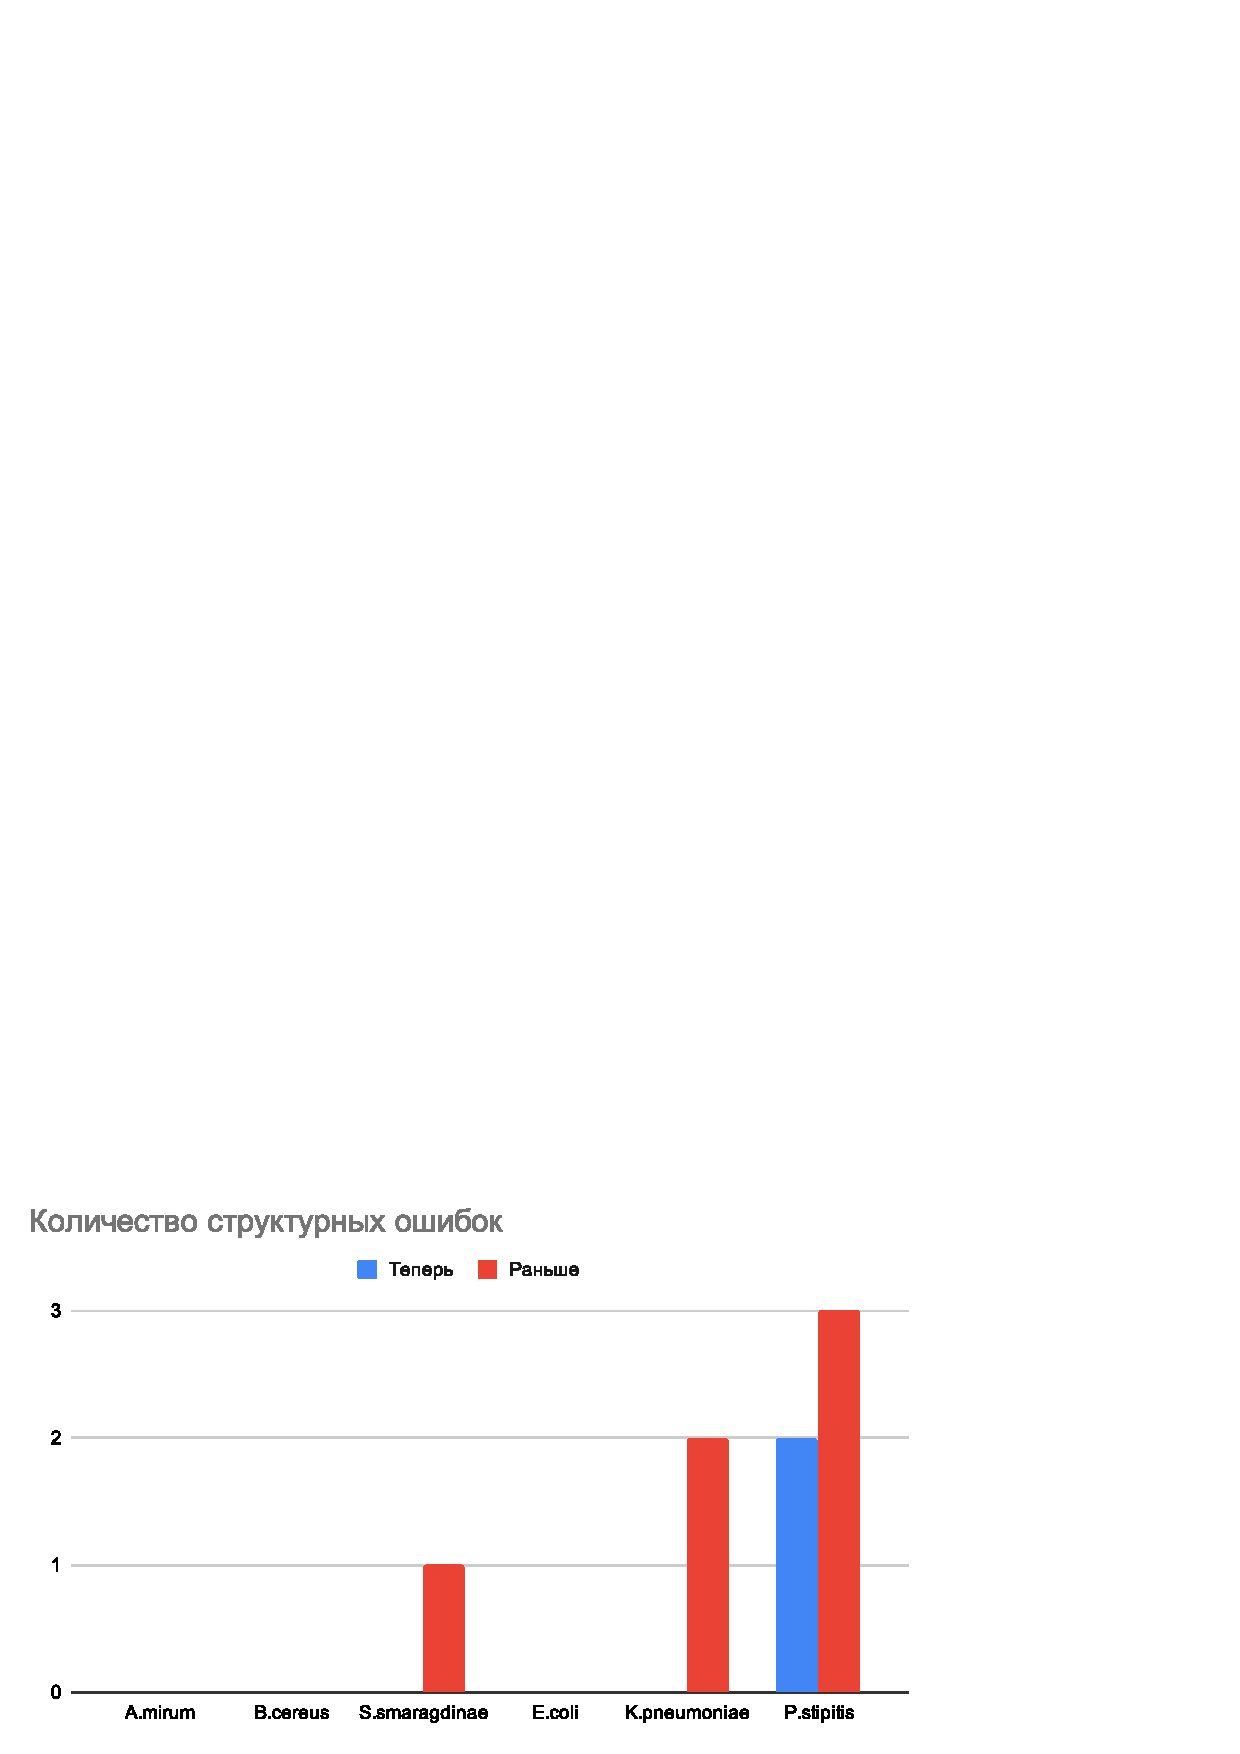
\includegraphics[scale=0.4]{misassemblies.png} 
	\caption{Дан контиг, состоящий из двух частей, расположение которых при сопоставлении с референсным геномом определяет тип структурной ошибки.}
  	\label{fig:miss}
\end{figure}


Уменьшение числа больших контигов означает, что удалось объединить несколько других больших контигов в один. Поэтому чем меньше значение данной метрики, тем лучше.

NGA50 контигов имеет смысл сравнивать относительно NGA50 самого референсного генома (потому что в геноме могут присутствовать несколько хромосом и плазмиды \cite{art:helinski2012plasmids}), и чем они ближе, тем лучше. В случае отсутствия значения для референсного генома можно считать, что чем большие значения NGA50 контигов, тем лучше. На всех графиках измерения представлены в миллионах bp.

\subsection{Сборки одиночных геномов}
В данном наборе тестов геномы собирались из ридов Illumina \cite{art:reads}. В качестве входных контигов использовался их референсный геном. Результаты некоторых сборок можно видеть на графиках \ref{fig:test1}.

\begin{figure}[h]
\begin{minipage}{0.5\textwidth}
	\centering
	\includegraphics[scale=0.55]{contigs1.eps} \small{(a) Количество больших контигов}
\end{minipage}
\begin{minipage}{0.5\textwidth}
	\centering
	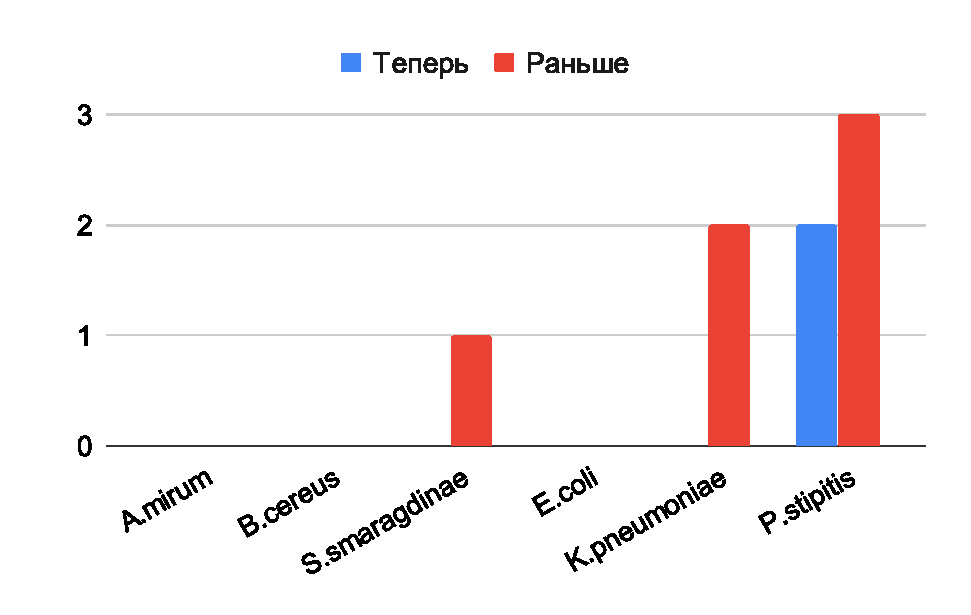
\includegraphics[scale=0.55]{mis1.eps} \small{(b) Количество структурных ошибок}
\end{minipage}
\begin{minipage}{0.5\textwidth}
	\centering
	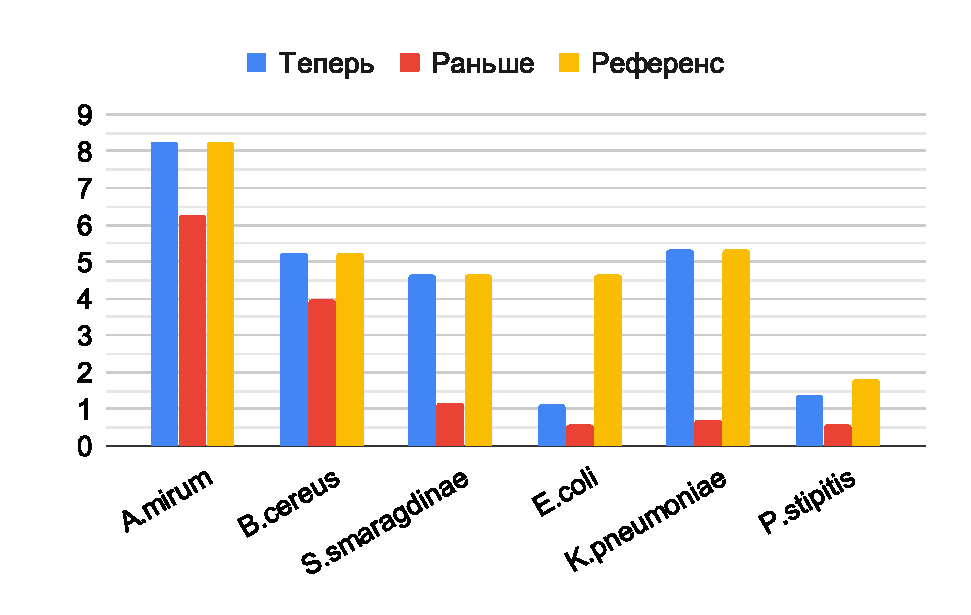
\includegraphics[scale=0.55]{nga1.eps} \small{(c) NGA50}
\end{minipage}
\begin{minipage}{0.5\textwidth}
	\centering
	\includegraphics[scale=0.55]{cov1.eps} \small{(d) Покрытие генома контигами}
\end{minipage}
\caption{Результат сборки одиночных бактерий}
\label{fig:test1}
\end{figure}

Стоит отметить, что P.stipitis --- это не бактерия, а гриб c девятью хромосомами. У грибов геном сложнее, чем у бактерий, поэтому граф сборки получается запутаннее, поэтому такое резкое ухудшение результатов по сравнению с остальными геномами ожидаемо.

\subsection{Использование стороннего ассемблера}
В данном разделе приводится пример сборки бактерии A.mirum с использованием двух ассемблеров: SPAdes и Flye \cite{art:flye}. Для сборки SPAdes использовались Illumina и Pacbio \cite{art:reads} риды, в то время как Flye использовал только PacBio риды. Затем производился запуск SPAdes с Illumina и PacBio ридами, но дополнительно в качестве контигов передавались результаты сборки Flye. Результат можно увидеть на графиках \ref{fig:test2}.

\begin{figure}[h]
\begin{minipage}{0.5\textwidth}
	\centering
	\includegraphics[scale=0.4]{contigs2.png} \small{(a) Количество больших контигов}
\end{minipage}
\begin{minipage}{0.5\textwidth}
	\centering
	\includegraphics[scale=0.4]{mis2.png} \small{(b) Количество структурных ошибок}
\end{minipage}
\begin{minipage}{0.5\textwidth}
	\centering
	\includegraphics[scale=0.4]{nga2.png} \small{(c) NGA50}
\end{minipage}
\begin{minipage}{0.5\textwidth}
	\centering
	\includegraphics[scale=0.4]{cov2.png} \small{(d) Покрытие генома контигами}
\end{minipage}
\caption{Сборка двумя ассемблерами бактерии A.mirum}
\label{fig:test2}
\end{figure}

Как видно из графиков, результат работы SPAdes можно значительно улучшить, даже если использовать не очень качественные результаты сборок других ассемблеров.

\subsection{Метагеномные сборки бактерий}
В этом разделе представлены результаты сборки метагенома, состоящего из 15 бактерий. Сборка производилась из Illumina ридов с дополнительной информацией в виде референсных геномов бактерий в качестве контигов. Результат можно увидеть на графиках на рисунке \ref{fig:test3}.
\begin{figure}[h]
\begin{minipage}{0.5\textwidth}
	\centering
	\includegraphics[scale=0.4]{contigs3.png} \small{(a) Количество больших контигов}
\end{minipage}
\begin{minipage}{0.5\textwidth}
	\centering
	\includegraphics[scale=0.4]{mis3.png} \small{(b) Количество структурных ошибок}
\end{minipage}
\begin{minipage}{0.5\textwidth}
	\centering
	\includegraphics[scale=0.4]{nga3.png} \small{(c) NGA50}
\end{minipage}
\begin{minipage}{0.5\textwidth}
	\centering
	\includegraphics[scale=0.4]{cov3.png} \small{(d) Покрытие генома контигами}
\end{minipage}
\caption{Результат сборки метагенома}
\label{fig:test3}
\end{figure}

Несмотря на то, что не во всех бактериях удалось получить меньшее количество больших контигов, главным результатом является значительное уменьшение количества структурных ошибок.

%==============================================================================
% У заключения нет номера главы
\newpage
\[\]
\newpage
\section*{Заключение}
В ходе данной работы были получены следующие результаты.
\begin{itemize}
    \item Разработан алгоритм скаффолдинга, использующего контиги.
	\begin{itemize}
		\item Алгоритм выравнивает контиги на граф сборки, а затем использует полученные пути при разрешении повторов.
	\end{itemize}
    \item Реализовано расширение для геномного ассемблера SPAdes.
	\begin{itemize}
		\item Реализовано на языке C++.
		\item Расширение позволяет эффективно использовать контиги в качестве входных данных.
		\item \begin{sloppypar} Исходный код SPAdes доступен по ссылке: \mbox{\url{https://github.com/ablab/spades/}}. Реализованное расширение будет доступно начиная с версии 3.15. \end{sloppypar}
	\end{itemize}
    \item Алгоритм протестирован на известных геномах.
	\begin{itemize}
		\item Протестировано на сборках одиночных геномов с высоким и низком качеством входных контигов, а также на метагеномной сборке.
		\item Теперь соединяется больше контигов с меньшим количеством ошибок по сравнению с предыдущим модулем SPAdes.
	\end{itemize}
\end{itemize}

%==============================================================================

\section*{Глоссарий}

\textbf{Ассемблер} --- программное обеспечение для получение контигов и скаффолдов из ридов.\\

\textbf{Граф де Брюйна} --- граф с параметром k, в котором рёбрами являются все возможные подстрок длины k+1 из некоторого набора строк, а вершинами --- перекрытия этих подстрок в k позициях.\\

\textbf{Граф сборки} --- в этой работе: граф, полученный в результате упрощения графа де Брюйна.\\

\textbf{К-мер} --- последовательность длины К.\\

\textbf{Покрывающий путь} --- путь, проходящий через заданное ребро.\\

\textbf{Плазмиды} --- небольшие молекулы ДНК, физически отделённые от хромосом.\\

\textbf{Референсный геном} --- эталонный геном данного вида организма.\\

\textbf{Риды} --- множество фрагментов ДНК, которые получаются в результате секвенирования.\\

\textbf{Контиги} --- восстановленные части ДНК из ридов.\\

\textbf{Скаффолд} --- объединение нескольких контигов с известным расстоянием между ними, но неизвестными самими нуклеотидами.\\

%==============================================================================

\setmonofont[Mapping=tex-text]{CMU Typewriter Text}
\bibliographystyle{ugost2008ls}
%\bibliographystyle{unsrt}
\bibliography{diploma}
\end{document}
